\chapter{Introduction}

\section{Exoplanets}  \label{sect:exoplanets}
Since the first detection of an exo-solar planet around a main sequence star 
\citep{mayor95},
the quest to find and study additional planets outside of our own solar system 
has been met with much enthusiasm and success. In recent years, numerous 
purpose-built instruments
%(e.g. \emph{HARPS}, \cite{mayor03}, 
%\emph{Kepler}, \& \emph{GPI} %\cite{macintosh14}) 
have been designed to detect exoplanets using a variety of methods, each with
their own unique sensitivities and biases. 
%For instance, the radial velocity (RV) method, which uses stellar spectra to 
%detect periodic Doppler 
%shifts in spectral features thus indicating the presence of 
%a companion, possibly planetary mass, is most sensitive to massive planets 
%with short orbital periods.  \\
Combining the results of multiple observational methods provides a global overview
of the planet population and thus provides insight into
the dominant pathways of planet formation and towards an understanding of how
common the conditions for life like our own are within our galaxy. \\

The results from many such dedicated exoplanet missions have been 
astounding. At the time of writing there are 3917 confirmed 
exoplanets\footnote{\url{https://exoplanets.nasa.gov/}; accessed on March 4, 2019.} 
with many thousands more planetary candidates. Furthermore, there 
exists a large diversity among planetary systems including the existence 
of certain exotic subsamples of exoplanets for which analogs do not exist within 
our own solar system. Some of these extreme systems include i) the so-called hot 
Jupiters (e.g. 51 Pegasi b; \citealt{mayor95}, HD 189733b; \citealt{bouchy05}, 
\& HD 209458b; \citealt{mazeh99, charbonneau00}): 
gas giant planets with masses comparable to or exceeding the mass of Jupiter  
but with orbital periods of $\lesssim 10$ days, ii) circumbinary planets (e.g. 
Kepler-16b; \citealt{doyle11}): 
planets which orbit stellar binaries, and iii) the most common planet types
in the local universe \citep{petigura13}, namely super-Earths and sub-Neptunes:
planets with radii between $\sim 1.5-4$ R$_{\oplus}$ with a range of orbital separations
(e.g. GJ 1214b; \citealt{charbonneau09}, Kepler 440b \citealt{torres15}, \&
K2-18b \citealt{foremanmackey15,montet15}).


\section{Methods of Detecting Exoplanets} \label{sect:detection}
Numerous methods for the direct or indirect detection of exoplanets
have been successfully demonstrated or proposed. All such methods provide complementary
access to the planetary parameter space thus enabling a unique view of the exoplanet
population. A non-exhaustive list of prominent exoplanet discovery methods follows.

\emph{Radial velocities}: measuring periodic variations in the doppler shift of star
around the barycenter of its planetary system due to the gravitational influence of
its planetary-mass companions. This method is used to measure the orbital separation of a
star and planet and place a lower limit on the planet's mass. The radial velocity
method favours the detection of massive short-period planets around inactive stars
(see Sect.~\ref{sect:rv} for more details).

\emph{Photometric transits}: monitoring the brightness of a star over time and
searching for periodically space brightness dips due to the occultation of the star
by an orbiting planet. This method is highly complementary to the radial velocity method
as it measures the planet's radius and orbital inclination where the latter can be
used to break the mass-inclination degenerancy suffered by radial velocity planet
detections. The recovery of radial velocity masses and transit radii together provide
views of planetary bulk densities which can be used to distinguish predominently
rocky planets from planets with significant size fractions of gaseous envelopes.
The transit method is the most successful planet detection as a single
wide-field camera can be used to montior many stars simulatenously and continuously.
However this method requries planets to have nearly edge-on orbits relative to the observer
and thus favours giant planets on close-in orbits.

\emph{Direct imaging}: spatially resolves planets from their host stars and thus
directly detects photons originating from the planet. The resulting planetary luminosity
measurements can be compared to forward models of planetary
evolution to infer planetary masses and possible formation pathways \citep{marley07}.
Multi-epoch observations can also reveal the properties on planetary orbits \citep{wang18}.
Due to the extremely small planet/star contrasts, direct imaging favours the detection
of young massive planets on wide orbits.


\emph{Transit timing variations}: or TTVs represent deviations in the expected transit
times of a transiting planet under the assumption of a linear ephemeris. Such deviations
may be attributed to an unseen planetary companion whose gravitational influence on the
transiting planet is observable either through close encounters or mean motion resonances.
The amplitude and periodicity of a transiting planet's TTVs can be used to constrain the mass
and orbital period of the perturbing planet.

\emph{Gravitational microlensing}:
offers a unique method for probing the planet population out to large distances
within the Milky Way as the detected photons do not originate from the planetary system itself
but rather from a distant bright source. As the gravitational field of a
foreground star (i.e. the lens) occults a distant bright source, the source appears to
brighten as a result of the lensing effect. In the case for which the len's gravitational
potential deviates significantly from radially symmetric as the result of an anomalous gravity
well, from say a planetary companion, that inhomogenity will distrupt the smoothness of the
len causing an anomalous brightening that reveals the presence of a co-moving companion with
a measurable mass. One drawback of this method is that observations of the same planetary
system are not repeatable.

\emph{Astrometry}: similarly to the radial velocity method wherein a planetary-mass companion
causes its host star to periodically wobble. The astrometry method is unique to the radial velocity
method as the observed variations occur in position space, rather than in velocity space, and
occur in the plane of the sky. This method is used to measure the orbital separation of a
star and planet and measure the planet's mass. Because the variation in the star's position
needs to be resolved, the astrometry method favours nearby planetary systems with massive
planets on wide-orbits.


\begin{figure}
  \centering
  %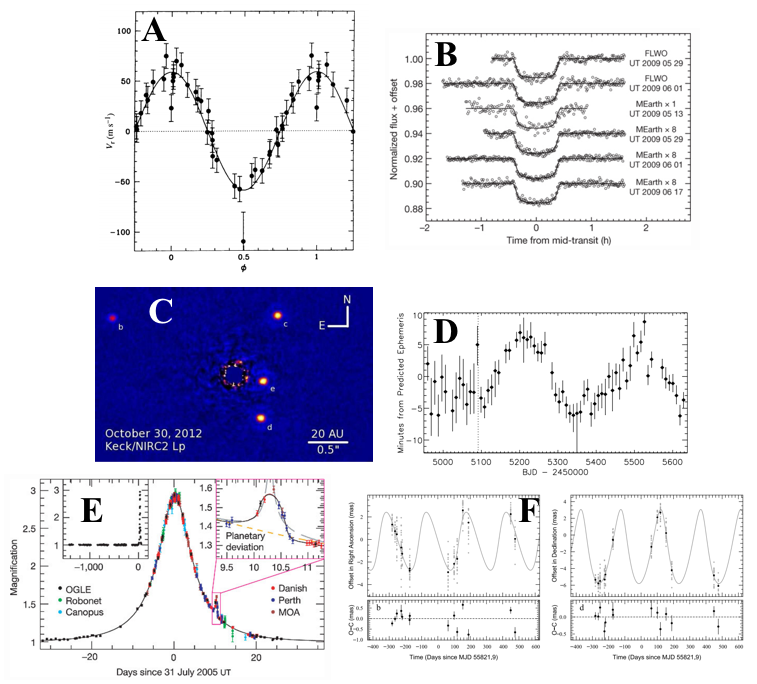
\includegraphics[width=\textwidth]{figures/detection_methods.png}
  \caption{Examples of observables for exoplanet detections using A)
    the radial velocity method \citep{mayor95}, B) planetary transits
    \citep{charbonneau09}, C) direct imaging \citep{currie14},
    D) transit timing variations \citep{ballard11},
    E) gravitational microlensing \citep{beaulieu06}, and
    F) astrometry \citep{sahlmann13}.}
  \label{fig:detection}
\end{figure}


\iffalse
\section{Potentially Habitable Planets} \label{sect:HZ}
One highly sought after result arising from the endeavour of exoplanet hunting 
is the detection of potentially habitable Earth-like planets. 
Broadly speaking, a potentially habitable Earth-like planet refers to 
an exoplanet whose bulk composition is known to be rocky and whose 
orbital period places the planet within a range of distances from its host star 
where we expect water on the planetary surface to exist in its liquid phase; 
the habitable zone (HZ) \citep{dole64, hart79}. Granted, this HZ 
definition is 
informed by our understanding of surface-based life on Earth and disregards 
the potential for additional, exotic forms of life such as water-based life 
in sub-surface oceans of planets. \\

Even with the limited definition of the 
HZ, it is known that numerous, and often unobservable factors complicate the 
exact definition of the HZ thus altering the expected orbital 
distances at which we should search for potentially habitable planets. 
Some of these factors include 

\begin{enumerate}
\item the presence of atmospheric greenhouse (GH) gases 
\citep{kasting93, kopparapu13} which 
absorb thermal radiation from the planetary surface and re-emit roughly as a 
blackbody thus heating the planetary surface to temperatures exceeding the 
radiative equilibrium temperature expected in the absence of an atmosphere. 
\item The presence of clouds \citep{selsis07, yang13} which increases the 
albedo thus causing the planet to be cooler than what is predicted by cloud-free 
models.
\item The planet mass \citep{kopparapu14}. Assuming an atmospheric composition 
that is dominated by greenhouse gases (i.e. H$_2$O and/or CO$_2$) and that the 
amount of atmospheric volatiles scales with the planet mass, the surface pressure 
can be written in terms of the atmospheric column density $N$ and planet's 
surface gravity $g$ as 

\begin{equation}
\frac{P_{\mathrm{s}}}{P_{\mathrm{s}, \oplus}} = \left( \frac{N}{N_{\oplus}} \right)
\left( \frac{g}{g_{\oplus}} \right).
\end{equation}

\noindent Adopting an empirically derived mass-radius relation for planets with 
$m_p < 5$ M$_{\oplus}$, e.g. $m_p \propto r_p^{3.2}$ \citep{kopparapu14}, 
the surface pressure increases with planetary mass as 

\begin{equation}
P_{\mathrm{s}} \propto m_p^{3/4}, 
\end{equation}

\noindent suggesting that more massive planets have thicker atmospheres.
\item Planetary rotation as the global atmospheric circulation dictates the 
spatial distribution of clouds. For instance, \citep{yang14} showed that 
slowly rotating planets can maintain hospitable climates over longer timescales than 
rapid rotators.
\item Relevant system geometries such as planet obliquity 
\citep{williams97, spiegel08, spiegel09} and orbital eccentricity 
\citep{dressing10, cowan12}. 
\end{enumerate}

This list of effects on planetary habitability represents a subset of the 
seemingly infinite (\textbf{exaggeration}) number of factors which determine 
whether or not an Earth-like biosphere can exist on an exo-solar planet. 
Luckily each of these properties can in principle be measured, at least for 
a subset of planets which are conducive to such observations. For example, 
for factors 1,2) above, 
the presence of particular chemical species and clouds/hazes 
in a exoplanetary atmosphere 
can be detected via variations in the apparent size of the planet as a function 
of wavelength; transmission spectroscopy \citep{seager00}, 3) the planet 
mass can be measured from radial velocities and/or transit timing variations 
\citep{holman05}, 4) the planetary rotation rate can be measured if the 
planetary spectrum can be distinguished from that of its host star and if the 
rotation rate is sufficiently large such that the rotational line broadening 
is detectable \citep[e.g.][]{snellen14, schwarz16}, and 5) the planetary obliquity or 
spin--orbit misalignment can be measured for transiting planets using 
spectroscopy \citep{rossiter24, mclaughlin24, queloz00} and their orbital 
eccentricities measured from radial velocities or secondary eclipse observations of 
transiting planets. \\

To date, a number of potentially habitable, Earth-like candidates have already 
been detected \citep[e.g. Kepler-438b, 442b;][]{torres15}). Although, these 
inferences of habitability are based on a limited number of arguments for the 
planet's size, mass,\footnote{Therefore its bulk density 
($\rho \propto m_p/r_p^3$) and surface gravity ($g \propto m_p/r_p^2$).} and 
insolation relative to Earth. Knowledge regarding the atmospheres and surface 
conditions of these planets still remains largely uncertain. Fortunately, 
atmospheric 
characterization is possible through techniques such as transmission and/or 
emission spectroscopy of transiting planets and near edge-on planets 
respectively. These methods have been successfully performed for a small 
sample of \emph{non-rocky} exoplanets only 
\citep[e.g.][]{bean13, crouzet14, kreidberg14, mccullough14}. 

\subsection{Adopted HZ Definition}
We opt to restrict our focus of HZ planets to the commonly used definition 
\citep{kasting93} and parametric model of \cite{kopparapu13}. 
In this definition the inner edge of the HZ 
is defined by the `moist GH' or `water-loss' limit wherein a slight increase 
in flux results in the 
photodissociation of water vapour and subsequent hydrogen escape in the upper 
atmosphere. The outer edge is then given by the `maximum GH' wherein any 
addition of CO$_2$ into the atmosphere results in a net cooling effect as the 
increased Rayleigh scattering (increased albedo) begins to dominate over the 
added GH effect resulting in a net cooling. \\

The parametric model \citep{kopparapu13} relates the orbital separations 
$a$ of the inner and outer edges of the HZ to the insolation received by planets 
at those distances. To compute the HZ edges for a given star requires its 
luminosity $L$ and effective temperature $T_{\mathrm{eff}}$ 
as input parameters. Specifically,

\begin{equation}
a = 1 \mathrm{\hspace{2pt} AU} \cdot \sqrt{\frac{L/L_{\odot}}{S_{\mathrm{eff}}}},
\end{equation}

\noindent where

\begin{equation}
S_{\mathrm{eff}} = S_{\mathrm{eff},\odot} + AT_* + BT_*^2 + CT_*^3 + DT_*^4,
\end{equation}

\noindent where $T_* \equiv T_{\mathrm{eff}}-5780$ K and the coefficients 
$S_{\mathrm{eff},\odot},A,B,C,D$ are computed for the `moist-GH' and `maximum-GH' 
limits (reported in \cite{kopparapu13}). This model is applicable to all 
early-to-mid M dwarfs and down to ultracool dwarfs with $T_{\mathrm{eff}}$ as 
low as 2600 K. \\

Finally we relate the orbital separations of the HZ edges to the observable 
orbital period $P$ using Kepler's third law:

\begin{equation}
P^2 \sim \frac{4 \pi^2}{G M_s} a^3.
\label{eq:keplersthird}
\end{equation}
\fi

\iffalse
Atmospheric transmission and emission spectroscopic techniques require 
bright host stars in order to acquire high signal-to-noise observations and is 
therefore naturally favoured by nearby targets. Therefore, to obtain  
atmospheric characterization of a rocky world with powerful upcoming 
instrumentation \citep[e.g. \emph{NIRISS} aboard \emph{JWST};][]{doyon12} we 
must first detect this population of nearby rocky exoplanets. To date, the 
highest priority terrestrial planet for atmospheric characterization is 
GJ 1132b \citep{berta15} at just 12 pc. Using the occurrence rates of small 
planets around M dwarfs from \cite{dressing15a}, they estimated that the 
nearest 
\emph{transiting} potentially habitable rocky planet is within 14.6 pc at 95\% 
confidence. GJ 1132b may therefore represent this planet. Integrating over 
planetary system inclinations, \cite{dressing15a} estimated that the nearest 
potentially habitable rocky planet is within just 3.5 pc at 95\% confidence. 
We have yet to discover such a planet but radial velocity efforts are 
currently being built and tested 
\citep[e.g. \spirou{;}][]{thibault12, artigau14} to achieve precisely this 
goal; finding the closest potentially habitable world. 
\fi

\section{Exoplanet detection via Stellar Radial Velocity} \label{sect:rv}
\subsection{Radial velocity curves}
The radial velocity (RV) method of detecting and characterizing exoplanets is largely
the focus of the work presented herein and so I provide an overview of its formalism. \\ 

The RV method represents a simple 
application of Newton's third law: `for every action, there is an equal 
and opposite reaction'. In this case, the presence of a planetary companion to a 
host star displaces the barycenter of the two-body system (i.e. the centre-of-mass) from the
centre of the star  itself. Because of this, a star with a sole companion 
will execute a keplerian orbit about the system's barycenter. The radial velocity of such a star
%as seen by any observer whose line of sight is not exactly orthogonal to the star's
%orbit normal,
is

\begin{equation}
V_r(t) = \gamma_0 + K[\cos{(\nu(t,P,T_0) + \omega)} + e\cos{\omega})],
\label{eq:rv}
\end{equation}

\noindent where $t$ is the independent time coordinate, $\gamma_0$ is the systemic velocity of
the star relative to the observer, $K$ is the semi-amplitude of the RV variation,
$P$ is the orbital period of the star and planet, 
$T_0$ is the reference epoch or time of inferior conjunction, and
the orbital elements $e$ and $\omega$ are the orbital eccentricity and argument of
periastron respectively. Note that $\omega$ is undefined for circular orbits with
$e=0$ and is assigned the conventional value of $\pi/2$ in such a scenario. \\

Eq.~\ref{eq:rv} is known as the keplarian orbital solution.
The true anomaly $\nu(t,P,T_0)$ defines the position of the star on its orbit 
relative to the argument of periastron and in the direction of motion. It is derived 
from another angular parameter, namely the eccentric anomaly $E(t)$. The eccentric 
anomaly can be solved for using the mean anomaly $M(t)$ according to 
Kepler's equation

\begin{equation}
M(t) = E(t)-e\sin{E(t)},
\label{eq:kepler} 
\end{equation}

\noindent where the mean anomaly is

\begin{equation}
M(t) = \frac{2\pi}{P} (t-\tau_{\mathrm{peri}}), 
\end{equation}

\noindent and $\tau_{\mathrm{peri}}$ is the epoch of 
pericenter passage. Because Eq.~\ref{eq:kepler} does not have a closed-form 
solution, in practice it is solved using iterative numerical techniques. 
Examples of keplarian orbits from Eq.~\ref{eq:rv} are shown in Fig.~\ref{fig:rv} 
for two 5 Earth mass planets each with an orbital period of 2 days around a 0.2 M$_{\odot}$ 
star. The first planet is on a perfectly circular orbit and therefore induces a purely
sinusoidal stellar RV curve while the second planet's eccentricity is 0.3 and exhibits a
RV curve that clearly differs from sinusoidal with the addition of the second cosine term in
Eq.~\ref{eq:rv}. \\


\begin{figure}
  \centering
  %\animategraphics[width=\textwidth,controls,loop]{150}{figures/RVcurve-}{0}{1}
  \caption{An animation of the orbits of two (non-interacting) planets of equal
    mass and on 2-day orbits around a 0.2 Solar mass star. One planet has a circular
    keplerian orbit ($e=0$) while the orbit of the other exhibits some ellipticity with
    $e=0.3$. The lower panel depicts the corresponding RV variation induced on the host star
    by each planet.}
  \label{fig:rv}
\end{figure}

The keplarian orbital solution is valid in the absence of dynamical 
perturbations to the two-body system. In this case only the true anomaly varies with 
time. However, if additional bodies are present in the system such as in binary star 
systems or in compact high multiplicity planetary systems, then the parameters in 
Eq.~\ref{eq:rv} need not be fixed and we instead refer to the measured orbit as the 
osculating orbit which may vary between orbital cycles. Note that if the timescale 
for perturbations to the stellar orbital solution is comparable to or less than the 
time interval over which radial velocity observations are taken, then the keplarian 
orbital solution in Eq~\ref{eq:rv} is insufficient and one must consider a more
complicated treatment of the dynamics typically in the form of N-body simulations.


\subsection{Fundamental planet parameters from the radial velocity method} \label{sect:K}
If we consider the simplest planetary system containing a star and a planet, each will 
orbit the system's barycenter or their common centre-of-mass (COM) whose position vector
is

\begin{equation}
\mathbf{r}_{\mathrm{COM}} = \frac{M_s \mathbf{r}_s + m_p \mathbf{r}_p}{M_s + m_p},
\end{equation}

\noindent where $M_s$ and $m_p$ are the stellar and planetary masses respectively and
$\mathbf{r}_s$ and $\mathbf{r}_p$ are their position vectors. 
Let us now take a barycentric view of this two-body system such that the 
COM coordinate is located at the origin ($|\mathbf{r}_{\mathrm{COM}}|=0$). Further
assuming circular orbits (i.e. $e=0$) and working 
in absolute scalar terms, the orbital distances of the star and planet are  
related via 

\begin{equation}
a_s M_s = a_p m_p,
\label{eq:com}
\end{equation}
  
\noindent where we have written $|\mathbf{r}_s|$ as $a_s$ and 
$|\mathbf{r}_p|$ as $a_p$. For a circular orbit, the stellar velocity around the COM has
the constant value

\begin{equation}
v_s = \frac{2\pi a_s}{P}.
\label{eq:velocity}
\end{equation}

\noindent As the star orbits the COM the maximum observed radial velocity of the star
is realized when the magnitude of the star's radial velocity vector
equals its velocity $v_s$. At these points in the orbit, $V_r(t)=v_s$ equals the semi-amplitude 
of the radial velocity curve $K$. Because the radial velocity 
curve, and hence $K$, is observable, 
we can relate $K$ to the masses of the star and planet by combining the velocity 
equation (Eq.~\ref{eq:velocity}) with the COM equation (Eq.~\ref{eq:com})
and Kepler's third law:

\begin{align}
\mathrm{max}(V_r(t)) = K &= \frac{2\pi a_s}{P}, \\
&= \frac{2\pi}{P} \left( \frac{m_p}{M_s} \right) a_p, \\
&= \frac{2\pi}{P} \left( \frac{m_p}{M_s} \right) \left( \frac{GM_s}{4\pi^2} \right)^{1/3} P^{2/3}, \\
&= \left( \frac{2\pi G}{M_s^2 P} \right)^{1/3} m_p. \label{eq:K1}
\end{align}

Eq.~\ref{eq:K1} contains two quantities which are directly observable from the RV time series.
Namely, the orbital period $P$ and semi-amplitude $K$. Observers will often seek an independent
constraint on the stellar mass $M_s$ from say the comparison of the stellar spectrum to
spectral templates of known spectral type and stellar mass from stellar evolution models
\citep[e.g.][]{muirhead12} or from
empirical relations between optical or near-IR stellar luminosities and dynamically
measured stellar masses \citep[e.g.][]{benedict16,mann19}. Prior knowledge of the
stellar mass enables the mass of the planetary companion to be inferred from the RV time series.
The uncertainties in the planet mass 
measurement are typically dominated by the noise in dataset which directly affects the
$P$ and $K$ measurement precisions but further uncertainties in $m_p$ are introduced by
uncertainties in $M_s$. \\

Looking more closely at Eq.~\ref{eq:K1} we can see that the RV semi-amplitude scales 
linearly with planet mass but has a negative scaling with stellar mass and orbital 
period. This makes sense because the RV effect is a manifestiation of a gravitational effect.
A larger perturbing mass (i.e. $m_p$) will result in a larger perturbation to the 
central body which itself becomes more difficult to perturb if more massive. Also the 
effect weakens when the distance between the bodies is increased (i.e. larger $P$). The 
RV method therefore has a natural observational bias towards massive, 
close-in planets around low mass stars. This explains why the first planets to be 
detected with the radial velocity method were hot Jupiters 
\citep[e.g.][]{mayor95}. For reference, the RV semi-amplitude that the Earth 
induces on the Sun is $\sim 9$ cm s$^{-1}$ whereas the $\sim 300$ times more massive Jupiter
induces a $\sim 12$ \mps{} effect despite having a factor of $\sim 5$ wider orbit.

\subsection{Caveats to Eq.~\ref{eq:K1}}
In the derivation of the RV semi-amplitude (Eq.~\ref{eq:K1}) we have neglected two 
important geometric effects. The first is that of eccentricity which, if non-zero, 
causes the stellar velocity to vary throughout the orbit such that
$\text{d}v_s/\text{d}t \ne 0$. Instead $\mathrm{max}(V_r(t)) > 2\pi a_s/P$ 
because the conservation of angular momentum requires that $v_s(\tau_{\text{peri}})$ 
be greater than elsewhere on the orbit. The corresponding correction 
factor to Eq.~\ref{eq:K1} is $(1-e^2)^{-1/2}$. \\

The second effect is that of inclination. When attempting to measure the planetary 
mass from RVs, the orbital inclination of the planetary orbit\footnote{Orbital 
inclination is conventionally measured  relative 
to the plane of the sky; i.e. an edge-on orbit has $i=90^{\circ}$.} is degenerate with
$m_p$ and is entirely unknown unless the planet has a well-defined transit model which is sensitive
to the orbital inclination. But the majority of planets are not transiting and hence have unknown
orbital inclinations. For these planets RV measurements 
are only sensitive to a mass lower limit $m_p\sin{i}$ rather than to the absolute planet mass.
The $\sin{i}$ correction factor also illustrates that an RV signal is only non-zero when
the observer's orientation is not exactly orthogonal to the normal of the star's orbital plane;
i.e. face-on orientations with $i=0$. \\

The inclusion of these correction factors gives a more complete description of the RV semi-amplitude: 

\begin{equation}
K = \left( \frac{2\pi G}{M_s^2 P} \right)^{1/3} \frac{m_p \sin{i}}{\sqrt{1-e^2}}. 
\label{eq:K2}
\end{equation}

\section{Measuring Radial Velocities} \label{sect:spectrograph}
\subsection{Stellar Spectroscopy}
Radial velocity variations induced by planetary companions cause the star to become 
periodically Doppler shifted. These wavelength shifts can be detected using hi-resolution 
spectroscopy as spectral features in the stellar photosphere are shifted from their 
rest wavelength $\lambda_{\text{rest}}$ as the star's velocity changes along the line-of-sight 
according to 

\begin{equation}
\frac{\Delta \lambda}{\lambda_{\text{rest}}} = \frac{V_r}{c},
\end{equation}

\noindent where $\Delta \lambda = \lambda_{\text{obs}}-\lambda_{\text{rest}}$ and
$\lambda_{\text{obs}}$ is the observed wavelength. 
In practice, velocity shifts are often measured from the cross-correlation of 
the observed stellar spectrum with a model or empirical template spectrum \citep{astudillodefru15}.
The highest precision is achieved when the results from many lines can be averaged. This makes
the RV method rather tractable for M dwarfs in particular which exhibit a plethora of 
spectral lines which become more abundant towards later type stars.
A sample of infrared spectra of early-to-late M dwarfs 
are shown in Fig.~\ref{fig:spectra} to demonstrate the wealth of absorption features. 
These spectra from \cite{rayner09} were obtained 
with SpeX at NASA's Infrared Telescope Facility at a resolving power of 
$R=\lambda / \Delta \lambda \sim 2000$. \\ 

\begin{figure}
\centering
%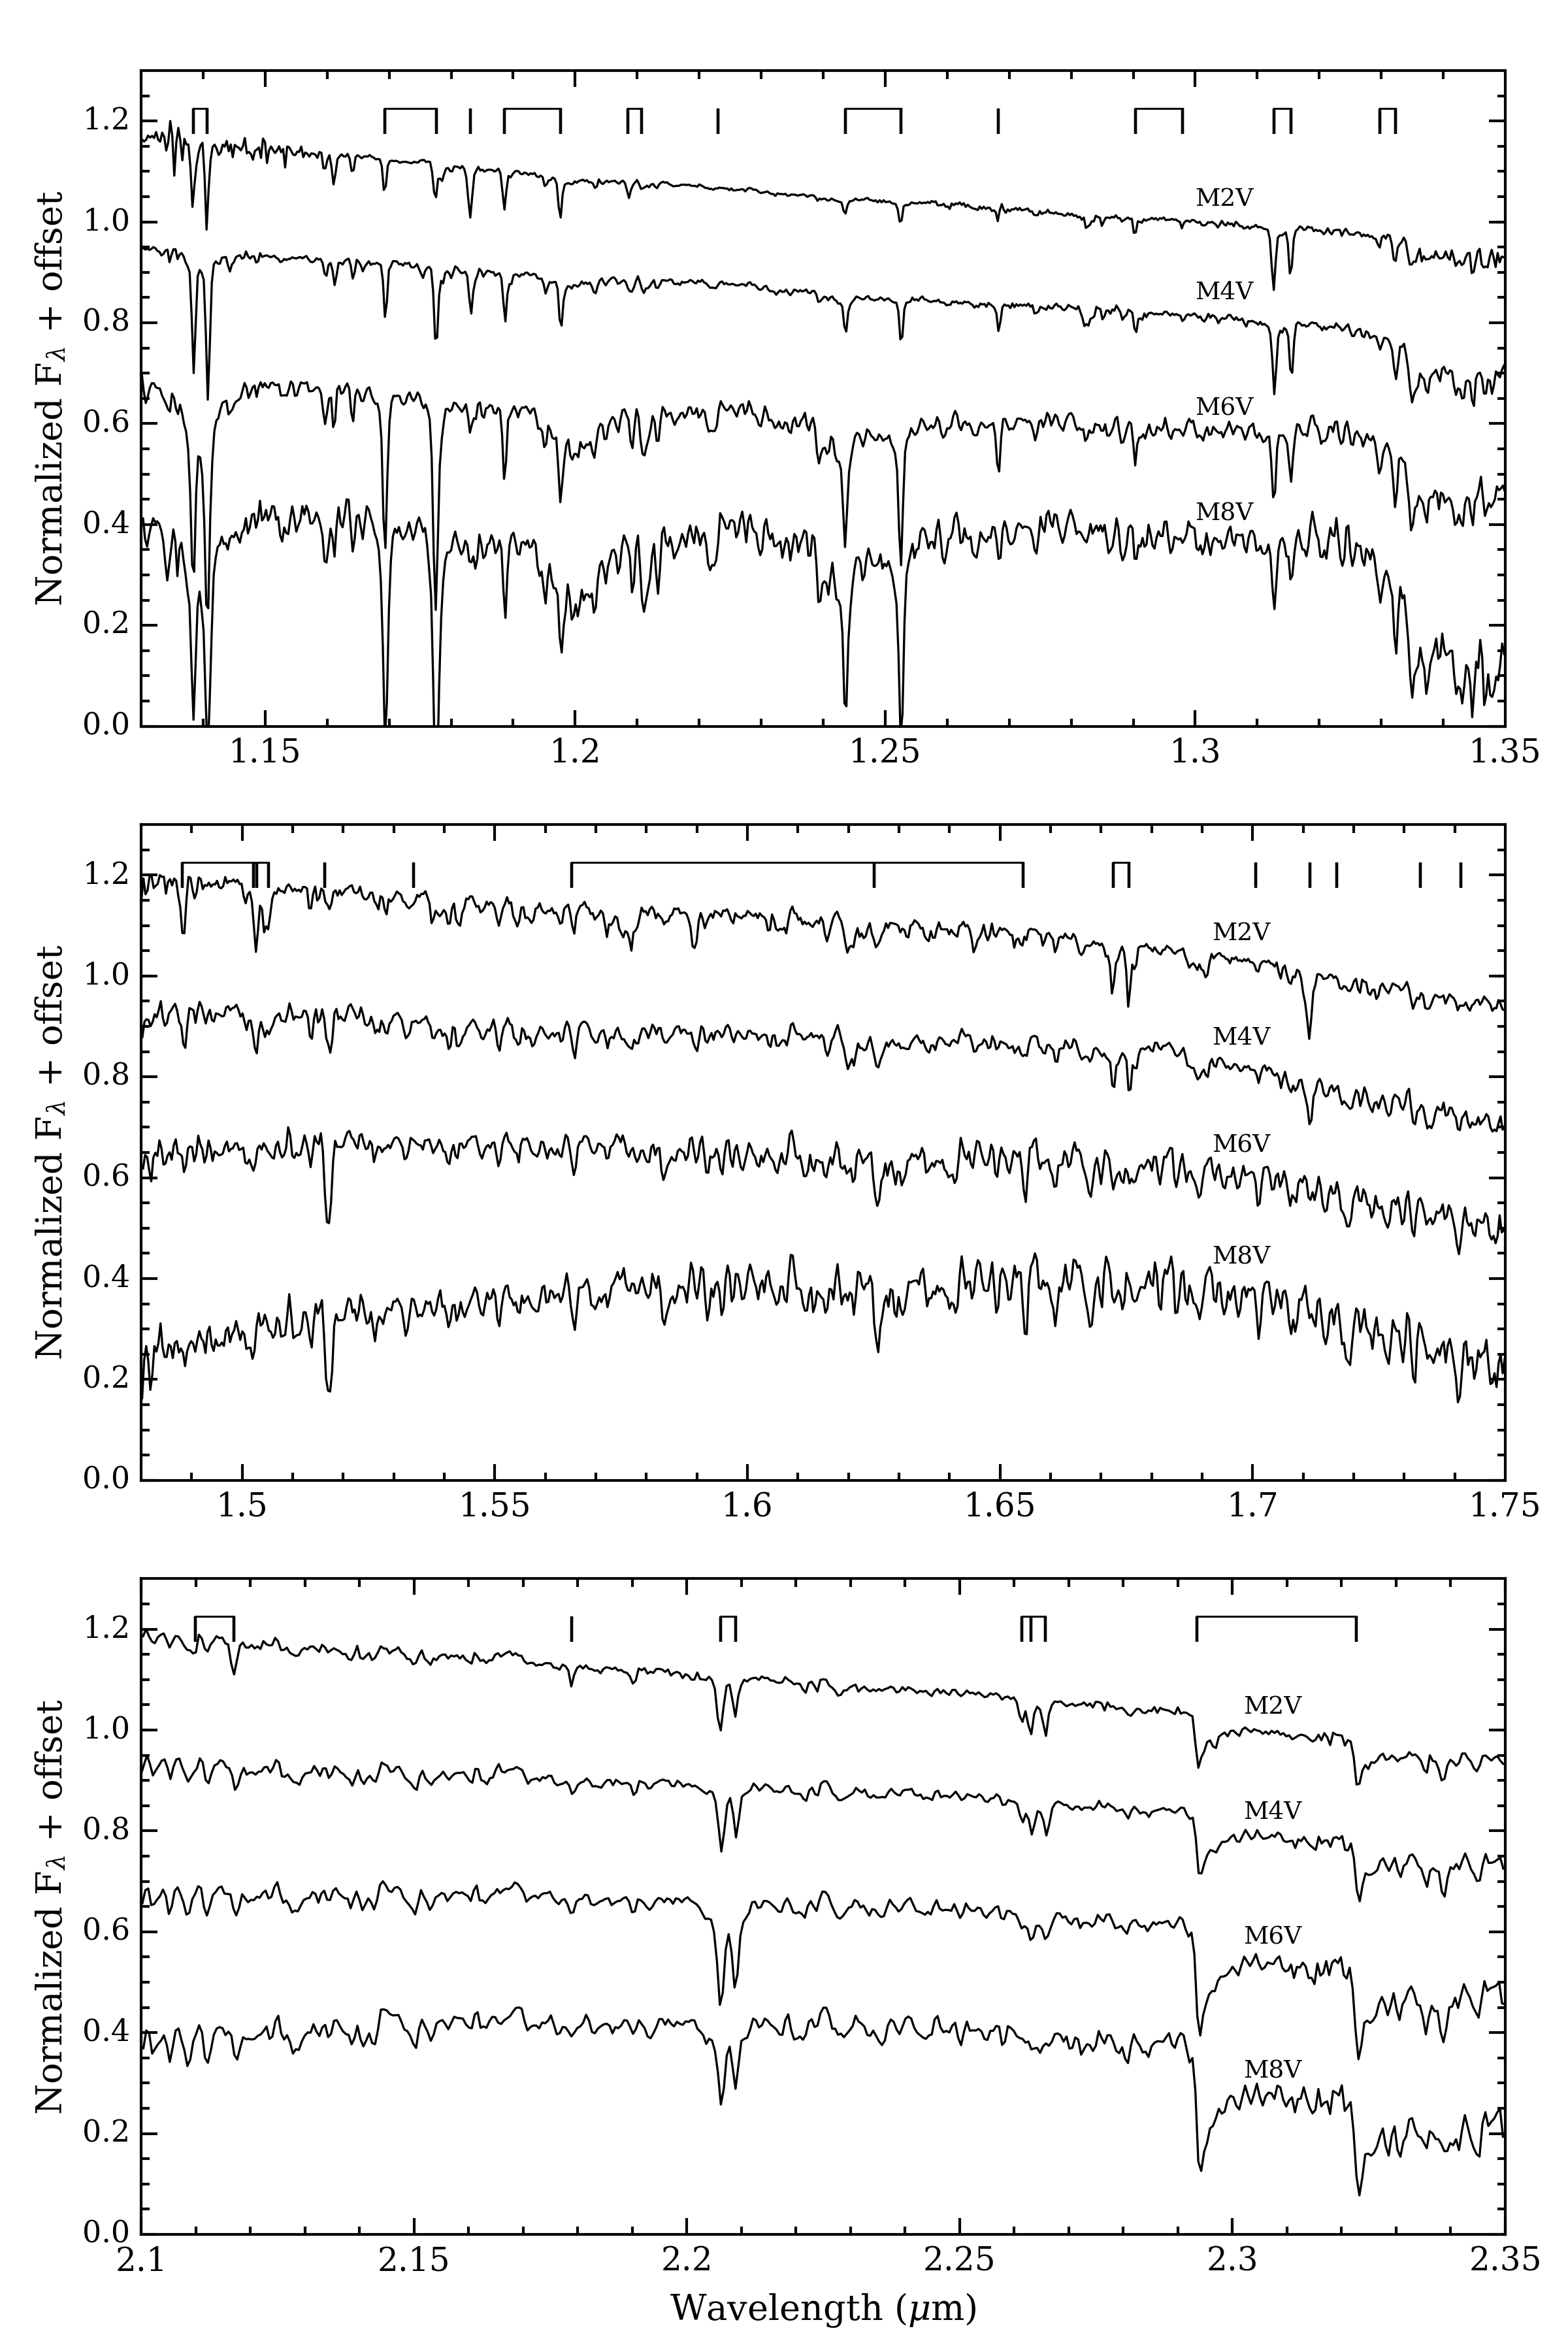
\includegraphics[scale=0.7]{figures/Mdwarf_spectra.png}
\caption{Medium resolution spectra of four early-to-mid M dwarfs in the J band (\emph{top}),
  H band (\emph{middle}), and K$_{\text{S}}$ band (\emph{bottom}) from the SpeX spectrograph
  at NASA's Infrared Telescope Facility. \label{fig:spectra}}
\end{figure}

The spectroscopic measurements are made with a spectrograph which contains a grating to 
diffract the incoming source light into its various colour components. Echelle spectrographs
in particular include an additional high order grating which separates the light into
spectral orders which are subsequently cross-dispersed spatially onto the detector. The dispersed
spectral orders create the observed stellar spectrum (Fig.~\ref{fig:harps}).
The spectrum is then cross-correlated with a  
template rest frame spectrum from the lab. The cross-correlation of prominent lines 
are averaged to create the cross-correlation function (CCF) of the star at the epoch of 
observation. The CCF is typically fit with a Gaussian line profile whose best-fit mean 
is equal to the measured radial velocity \citep{pepe02}. 
Active regions on the stellar surface arising 
from the presence of magnetic fields can have additional effects on the observed CCF 
causing the line profile to be exhibit non-Gaussianities. 
As we shall see in Sects.~\ref{sect:fwhm} and \ref{sect:bis}, these distortions can 
be used to model the stellar activity which can then be subtracted to possibly reveal 
any present planetary signals in radial velocity.

\begin{figure}
  \centering
  %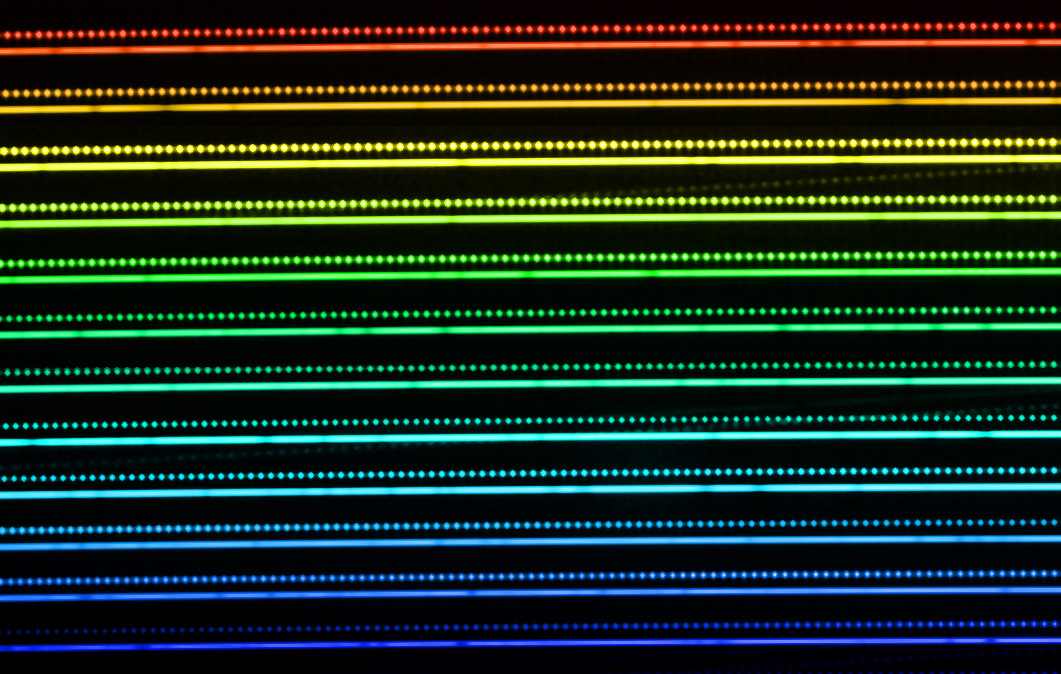
\includegraphics[scale=0.5]{figures/20140904_harps-lasercomb.jpg}
  \caption{A colourized image of the HARPS detector showing a subset of its 72 spectral orders.
    Each row pair contains the stellar spectrum (solid spectrum) over a portion of the HARPS wavelength
    domain and the corresponding wavelength reference from its laser frequency comb (dotted spectrum).
    Accurate wavelength calibration enables monitoring of stellar absorption features over time which
    may reveal periodic Doppler shifts possibly indicative of a planetary companion.
    Image courtesy: \emph{European Southern Observatory}.}
  \label{fig:harps}
\end{figure}

\subsection{Radial Velocity Error Budget Overview}
\subsubsection{Instrumentation Challenges}
Numerous sources of uncertainty hinder an observer's ability to measure infinitesimally precise
RVs from an observed spectrum \citep{podgorski14,halverson16}.
Many of these issues are intrinsic to the experimental
hardware. A non-exhaustive list of prominent issues with RV spectrographs includes

\begin{itemize}
\item thermal stability,
\item pressure stability,
\item wavelength calibration,
\item vibration control,
\item detector imperfections (i.e. readout noise, intrapixel quantum efficiencies, etc),
\item scattered light,
\item fiber modal noise,
\item tracking errors,
\item focus errors, and
\item atmospheric dispersion.
\end{itemize}

\noindent The aforementioned sources of error arise from the design and operation of the
instrument and telescope. As such, their mitigation is set by the specifications of the instrument
and cannot be improved by any post processing. 

\subsubsection{Photon noise limit}
The photon noise limit represents the fundamental limit to the RV measurement precision that can
be obtained from a stellar spectrum $A_i$. Here $i$ is the index over wavelength elements.
The photon noise limited RV precision from \cite{bouchy01} is

\begin{equation}
  \sigma_{\gamma} = \frac{c}{\text{S/N} \cdot Q}
\end{equation}

\noindent where $c$ is the speed of light, S/N is the signal-to-noise of the spectrum over its
complete spectral domain, and

\begin{equation}
  Q = \frac{\sqrt{\sum_i W_i}}{\sqrt{\sum_i A_i}}
\end{equation}

\noindent is known as the quality factor and represents the density of RV information content
in the spectrum $A_i$ measured in photoelectrons. The weighting function is given by

\begin{equation}
  W_i = \left( \frac{\lambda_i^2}{A_i} \right) \left( \frac{\partial A_i}{\partial \lambda_i} \right)^2.
  \label{eq:weight}
\end{equation}

By the dependance of $\sigma_{\gamma}$ on the first spectral derivative of the observed spectrum
(Eq.~\ref{eq:weight}), high S/N spectra with a high density of sharp features will provide the
best possible RV precision. Because the sharpness of the lines is important, obtaining high
resolution spectral has a direct benefit on minimizing $\sigma_{\gamma}$. Similarly stars
with low levels of collisonal and rotational broadening (i.e. low $\log{g}$ and \vsini{)} are
favourable targets for minimizing $\sigma_{\gamma}$. Also because line density is important, cooler stars
with a high metallicity are favourable as they exhibit more molecular and metal features.
Fig.~\ref{fig:sigrv} demonstrates these dependancies over the spectral
bands $UBVRIYJHK_{\text{S}}$.

\begin{figure}
  \centering
  %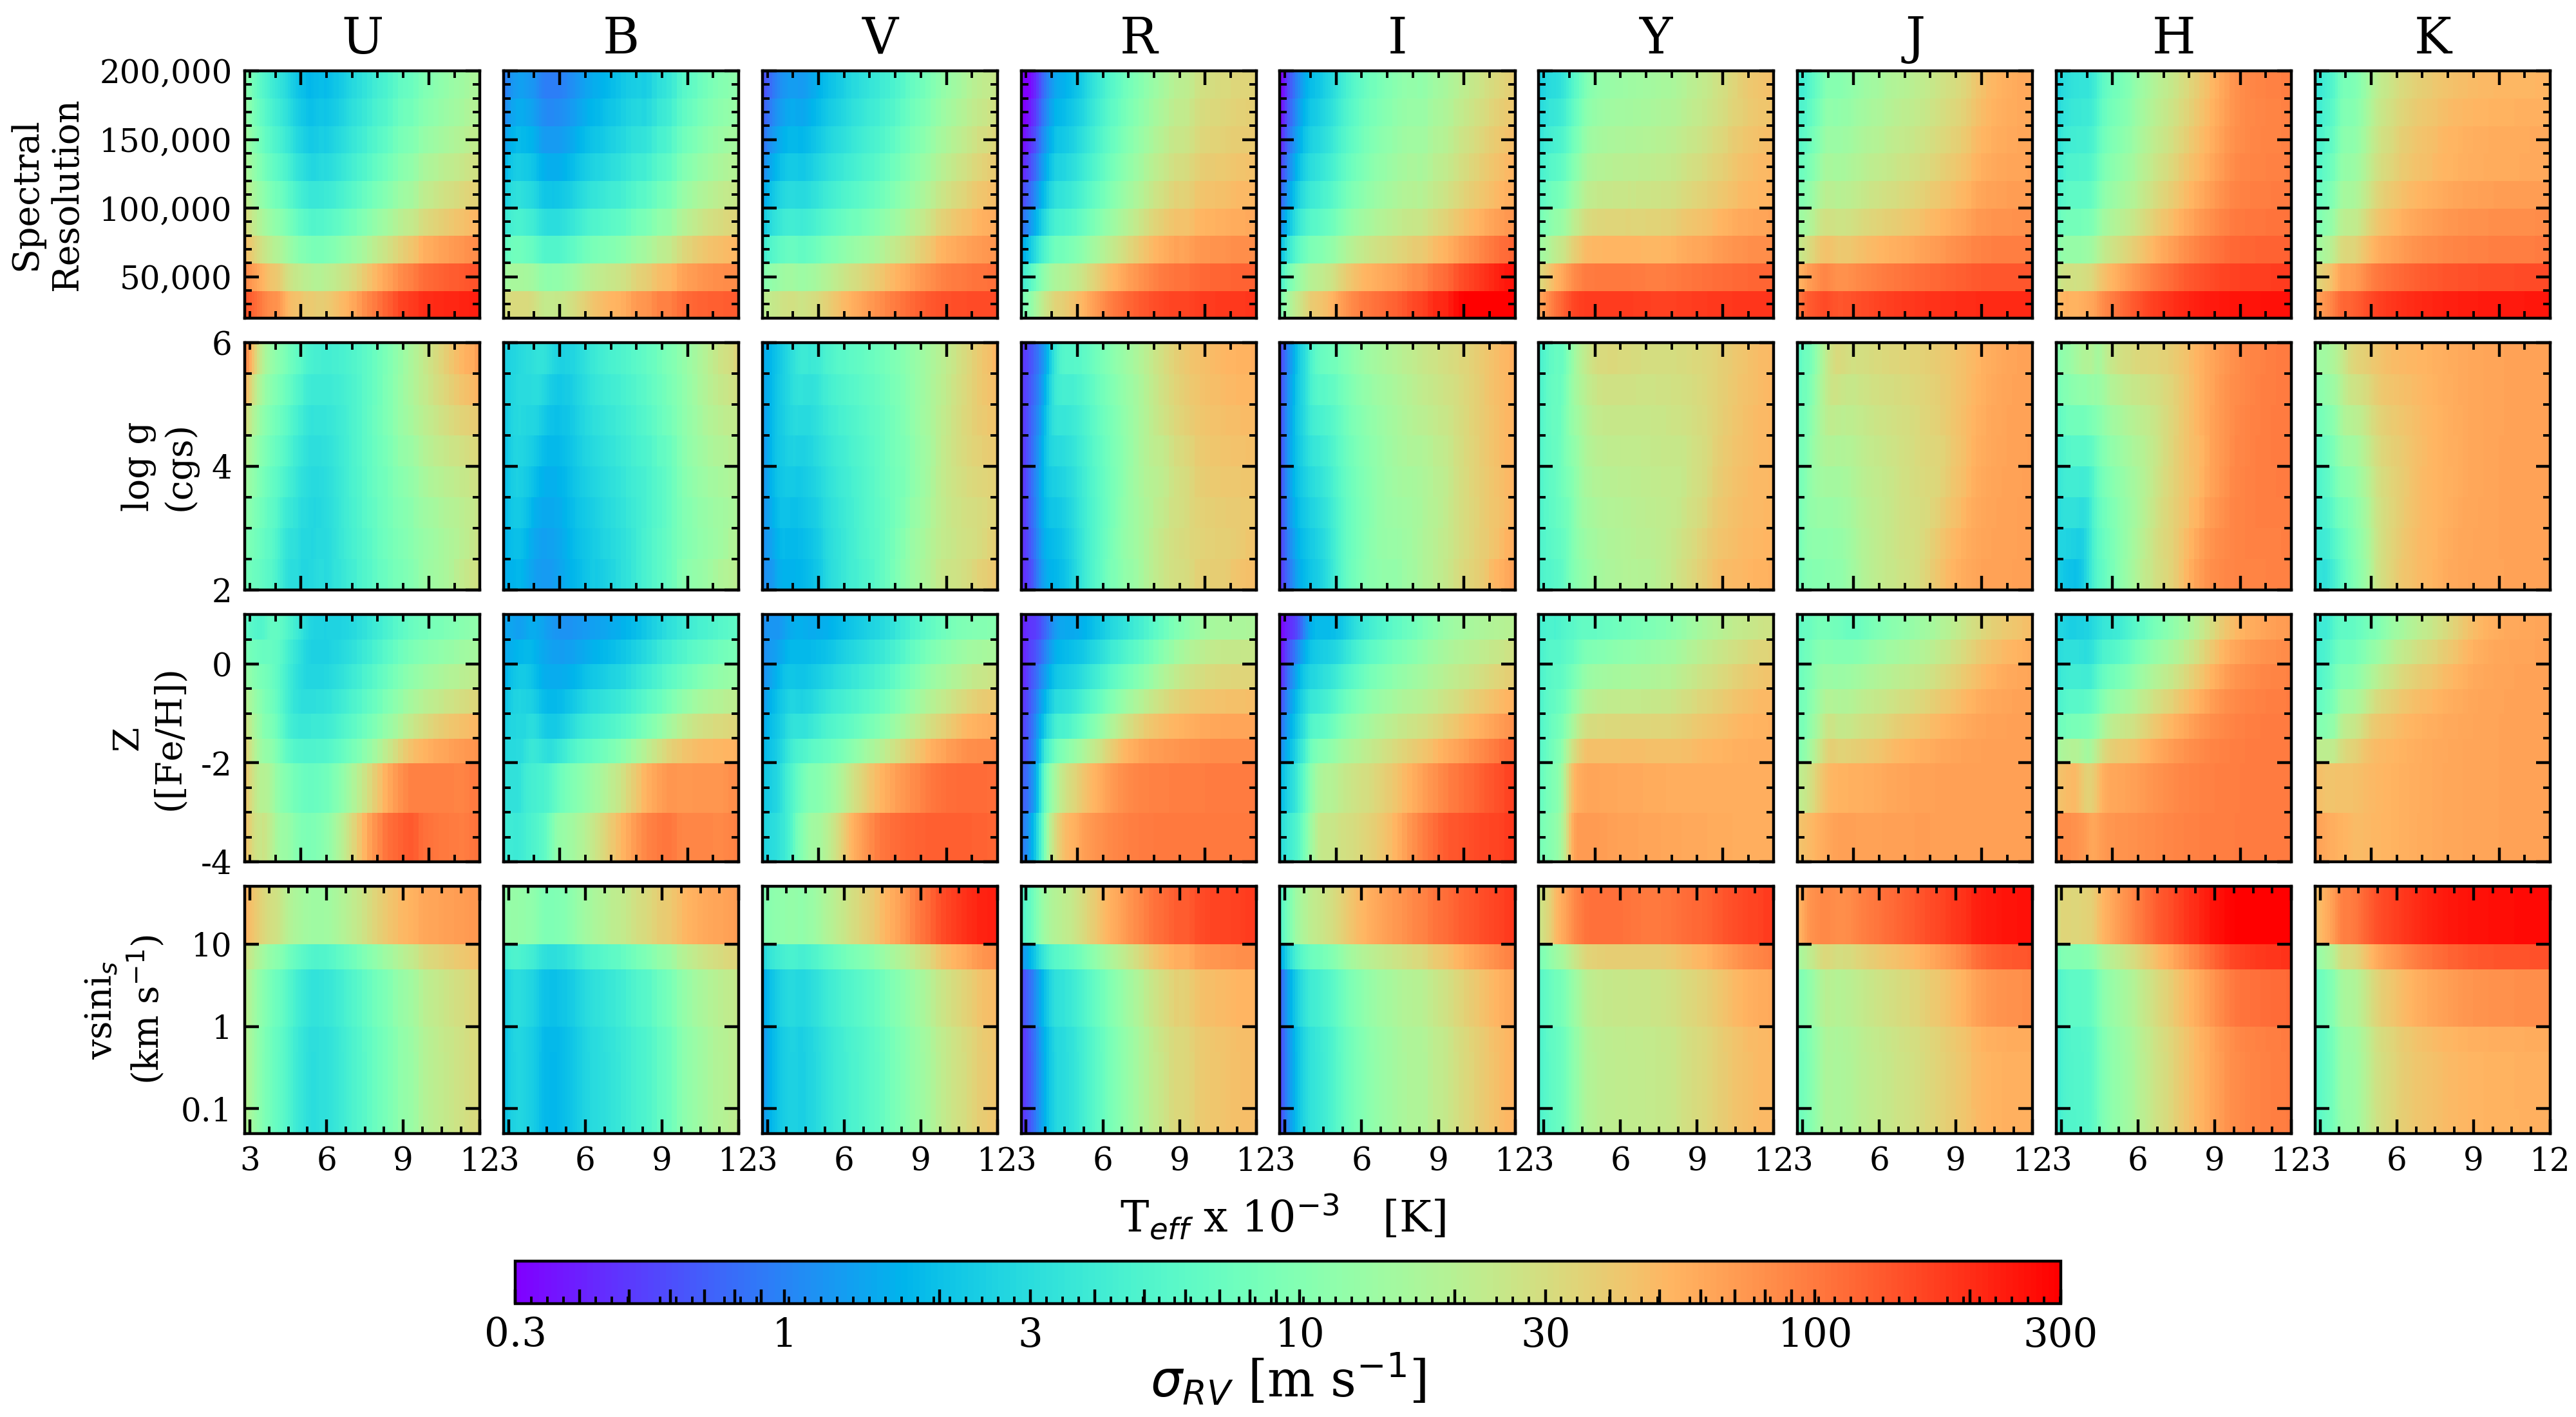
\includegraphics[width=\textwidth]{figures/sigRV_grid.png}
  \caption{Distributions of the photon noise limited RV precision in the $UBVRIYJHK_{\text{S}}$
    bands and as a function of spectral resolution, $\log{g}$, metallicity, \vsini{,}
    and stellar effective temperature. The distribution shown in each subpanel is marginized
    over all parameters not depicted on either of the panel's axes.}
  \label{fig:sigrv}
\end{figure}

\subsubsection{Telluric contamination}
In addition to errors arising from the instrumentation, there are also physical sources of RV
uncertainty that need to be accounted for in the post-processing software. One example is the effect
of telluric contamination of the observed spectrum by spectral features origining from Earth's
atmosphere. Because all high precision RV experiments are executed from the ground the incoming
starlight must traverse much of the Earth's atmosphere at which time telluric features become
imprinted on the incident spectrum. This effect is much more prominent in the infrared where
the atmosphere becomes much more opaque than in the visible in large part due to absorption by
atmospheric water vapour (Fig.~\ref{fig:transmission}). In the visible, small regions
in wavelength space that are known to be contaminated by tellurics can be simply masked without
significant loss of RV content. Whereas this method if applied to near-IR spectrographs would
eliminate so much RV information that it would negate any benefits of developing near-IR RV
spectrographs at all. Instead, near-IR RVs will need to rely on more sophisticated data-driven
methods of telluric spectrum extraction \citep[e.g.][]{artigau14,bedell19}.

\begin{figure}
  \centering
  %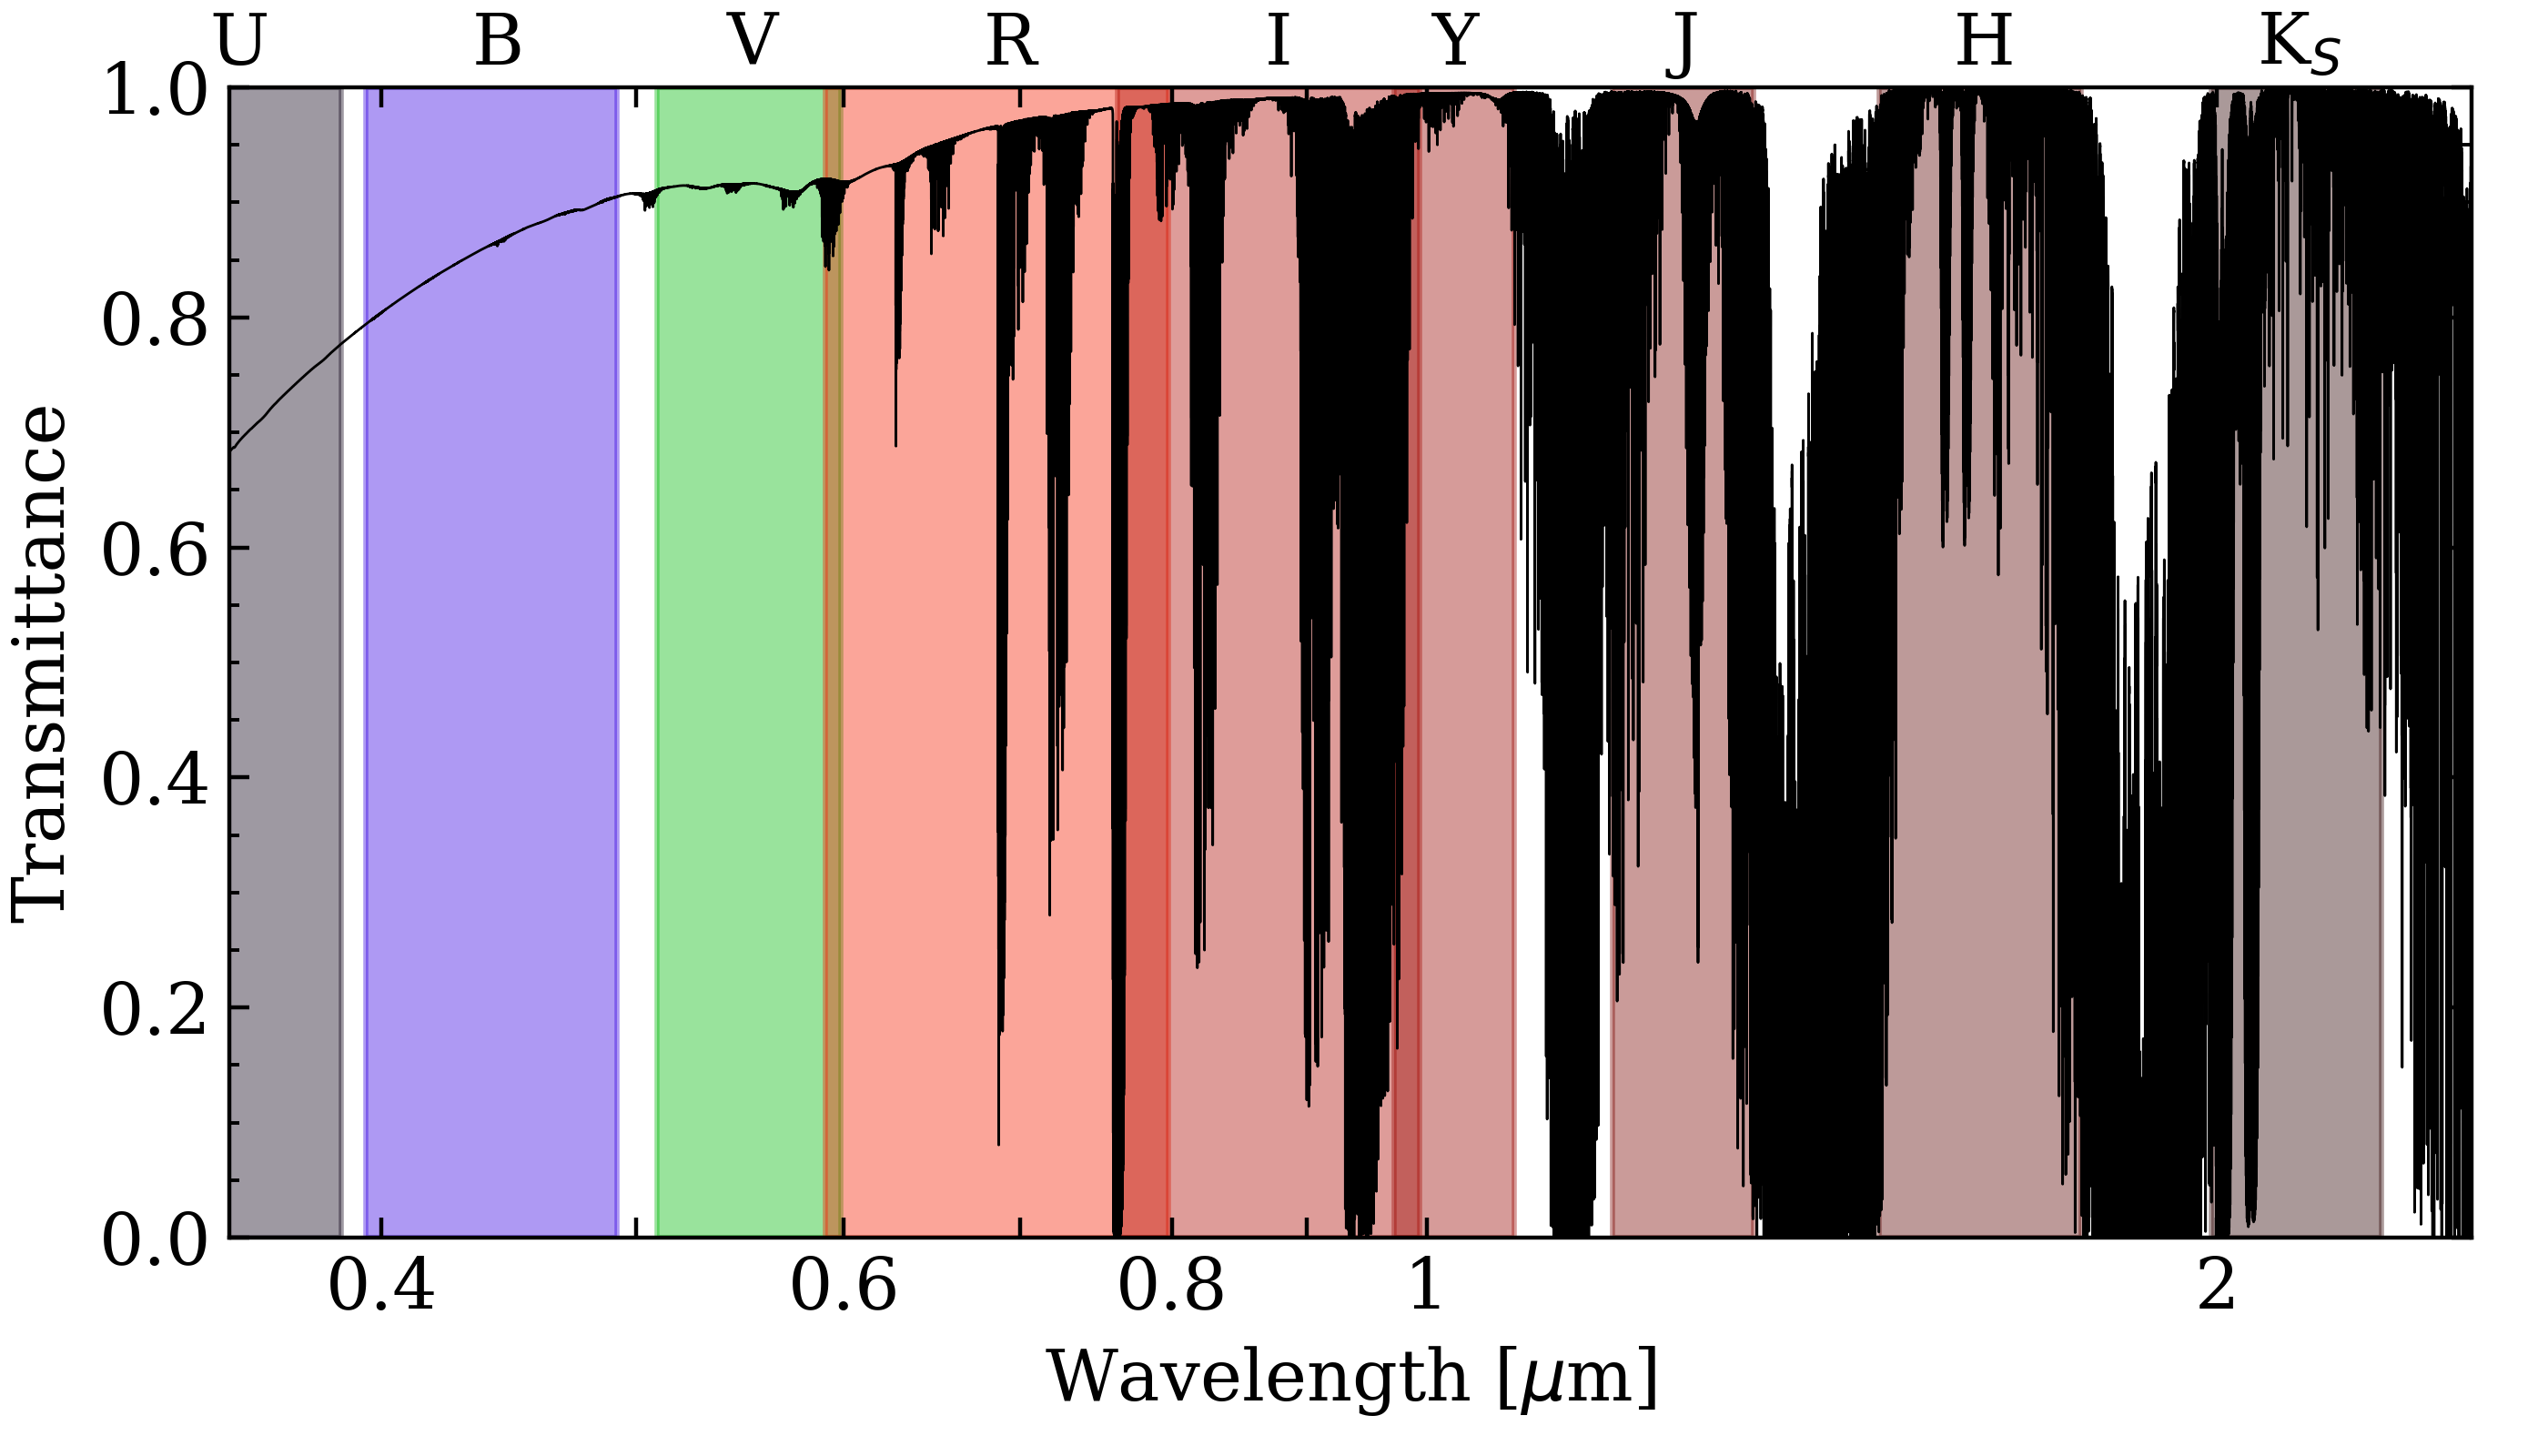
\includegraphics[width=\textwidth]{figures/transmittance.png}
  \caption{A \texttt{TAPAS} model of the radiative transmittance through the Earth's atmosphere
    as seen from MaunaKea at an airmass of unity \citep{bertaux14}. It is clear that the atmosphere
    becomes increasingly opaque towards infrared wavelengths with small observing windows at the
    $YJHK_{\text{S}}$ bands.}
  \label{fig:transmission}
\end{figure}

\subsubsection{Stellar activity} \label{sect:activity}
There exists a variety of physical processes in the photospheres and chromospheres of stars that
can lead to temporally correlated RV signals which are collectively
referred as \emph{stellar activity}. Alternatively, activity sources that act on short timescales
(i.e. seconds to minutes) are sometimes referred to as stellar jitter.
Particularly in RV planet studies, stellar activity
signals are the bane of observers because their signals can mask and
in certain instances even mimic the planetary signals that we are searching for. \\

Depending on the exact physical process these
signals can have widely differing timescales and manifestations in
spectroscopic, photometric, and polarimetry observations. In general, activity
signals are also wavelength dependent unlike Doppler variations induced by
planetary companions. Ancillary time series to RV measurements
derived from any of the aforementioned observations can therefore be used to
disentangle stellar activity from achromatic Doppler shifts induced by a companion.
Examples of sources of stellar activity are summarized in the subsequent paragraphs
while a brief summary is given in Table~\ref{table:activity}. \\

\begin{table*}
\small
\renewcommand{\arraystretch}{0.7}
\caption[]{Summary of Radial Velocity Stellar Activity Sources}
\label{table:activity}
\begin{tabular}{cccl}
  \hline \\ [-1ex]
  \textbf{Activity} & \textbf{Typical} & \textbf{Typical Signal} & \textbf{Notes} \\
  \textbf{Source} & \textbf{Timescale} & \textbf{Amplitude} & \\
  \hline
  Flares & a few minutes & tens of \mps{} & Has distinct photometric and spectroscopic signatures. \\ 
  &&&Observations during a flaring event should be excluded \\
  &&& from planet searches$^1$. \\
  \hline
  Oscillations & tens of minutes & few \mps{} & Can be mitigated with sufficiently long exposure times \\
  &&&or multiple observations per night$^2$. \\
  \hline
  Granulation & tens of minutes & few \mps{} & See oscillations.  \\
  \hline
  Active Regions & few stellar & sub-\mps{} $\to$ & Timescale and amplitude depend heavily on the active \\
  & rotation periods & tens of \mps{} & region sizes and on stellar rotaton$^3$. See Fig.~\ref{fig:rotation} for \\
  &&& the distribution of M dwarf \prot{.} \\
  \hline
  Magnetic Cycles & $\sim  7-30$ years & tens of \mps{} & Is only important when searching for \\
  &&&long period planets.
  \end{tabular}
\begin{list}{}{}
\item {\bf{Notes.}}
      $^{1}$ \cite{reiners09}, $^2$ \cite{dumusque11a}, $^3$ \cite{dumusque11b}. \\
\end{list}
\end{table*}


\emph{Flares}: magnetically active stars can undergo energetic flares or coronal mass
ejections originating from the stellar atmosphere. The exact flare physics
in M dwarfs is still uncertain but clearly requires strong magnetic fields
which can be sustained by turbulent convective motions and rotation
\citep{browning08}. Flare events are easily identifiable as they
exhibit a characteristically rapid increase in brightness (or in the intensity
of certain emission lines; e.g. Ca II, He I, H$\alpha$, etc. \citealt{schmidt12})
followed by an exponential decay over hours. Because RV
measurements affected by flares can be easily identified by the characteristic
line intensity spike over short time scales, such measurements are commonly
removed from planet searches \citep{reiners09}. \\

\emph{Stellar Oscillations}:
small scale mechanical perturbations to the internal stellar structure
can give rise to oscillation modes. If not damped, these oscillations
can propagate through the stellar interior before rebounding at the surface
of the star thus creating observable pulses in brightness and in the RVs of a
few \mps{} on a time scale of a few to tens of minutes \citep{bedding01}. 
This phenomenon is predominantly observed in Sun-like and post main sequence stars.
Due to the short timescale of
pulsation variations in radial velocity measurements of pulsating stars, the
jitter is mitigated through the use of sufficiently long exposure times
\citep{lovis05, dumusque11a}. \\


\emph{Granulation}:
stars with outer convection zones like the Sun and M dwarfs, exhibit granulation
at their surface. The granulation pattern is the result
of convection cells penetrating the surface; hot fluid parcels rising to the surface before
cooling and descending back into the stellar interior (see Fig.~\ref{fig:granulation}).
These patches of hot rising fluid are brighter than the regions of cold descending fluid.
Furthermore, the relative fractional coverage of a star's surface by rising fluid parcels is
in general greater than that of descending ones as evidenced in Fig.~\ref{fig:granulation}.
Along the line-of-sight, the RV component of photons emitted by the rising parcels at the
photospheric boundary will be blueshifted whereas the receding fluid within the
`intergranular lanes' will be redshifted. The domination of the stellar
surface area by hot parcels results in a granulated star having a net \emph{convective
  blueshift}. \\

\begin{figure}
  \centering
  %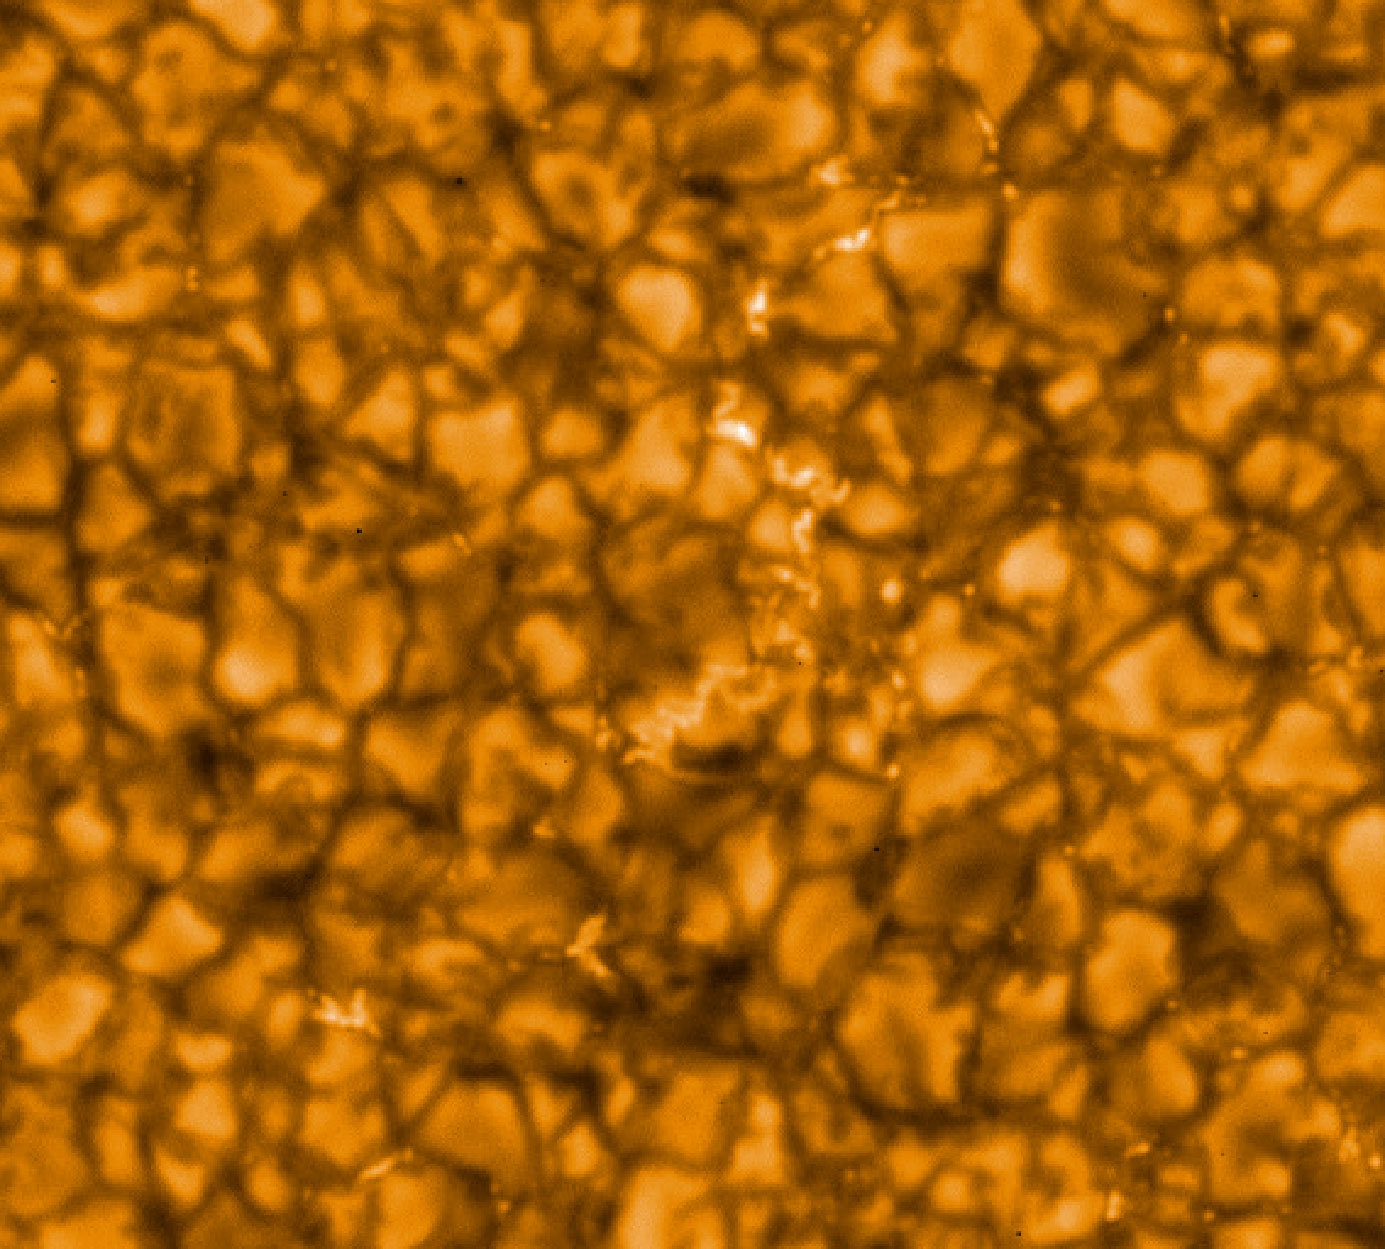
\includegraphics[width=0.8\textwidth]{figures/solargranulation.jpg}
  \caption{An image of a patch of the solar surface taken with NASA's Hinode Optical
    Telescope. The bright regions are the result of rising hot fluid parcels whereas the cooler,
    `intergranular lanes' reveal where the gas has cooled and descends back into the solar
    interior. (Image credit: Hinode JAXA/NASA/PPARC)}
  \label{fig:granulation}
\end{figure}


The short lifetimes of \emph{typical} granules
\citep[$\sim 10$ minutes;][]{hall08,gilliland11}) implies that brightness variability of the
surface varies on a similar timescale.
%Such variations have been measured using high cadence photometry
%\citep[e.g.][]{gilliland11}.
The corresponding RV jitter is dependent on the relative velocity of convective
cells across the stellar surface. Noting that the relative sizes of granules varies over time, so
too does the resulting RV jitter whose \emph{net} effect (hot and cold regions partially
cancel each other) is typically at the level of a few \mps{} \citep{lindegren03}. \\
%This level of radial
%velocity jitter has been observed on both the Sun \parencite{kuhn83} and on $\alpha$ Cen A
%\parencite{kjeldsen99}. \\

\emph{Active Regions}:
like the Sun, the photospheres of active late-type stars are often littered with active regions such
as dark star spots and/or hot faculae or plages in the chromosphere. These localized regions of either
hot or cold gas relative to the surrounding photosphere become trapped by magnetic field loops reconnecting
with the stellar surface. Active regions create a temporally evolving
RV signal and spectral line profile distortion due to their unique emitting temperatures and their orientation
as they rotate in and out of view (see Fig.~\ref{fig:starspot}). In the Sun, these structures
have long been known to be associated with strong local magnetic fields as evidenced by the observed
Zeeman splitting (see Sect.~\ref{sect:zeeman}) of lines emitted from these active regions
\citep{hale08}. \\

\begin{figure}
  \centering
  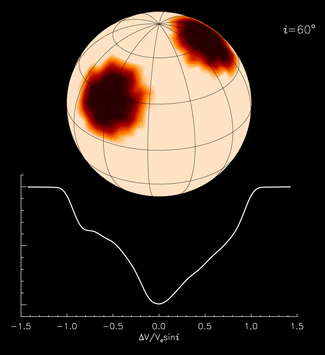
\includegraphics[scale=.8]{figures/starspot.png}
  \caption{An snapshot example of a spotted stellar photosphere and its effect on the disk-integrated
    spectral line profile. The cool spots disrupt the symmetry of the
    line profile according to the temperature difference between the spot and
    unspotted photosphere at its position on the stellar disk.
    \citep[Image credit:][]{kochukhov16}}
  \label{fig:starspot}
\end{figure}

The activity timescale from active regions is modulated by the stellar rotation. The stellar rotation
period \prot{} can often be measured for active stars with non-zero
inclination from the quasi-periodicity of its photometric variability.
The spectroscopic method of measuring a star's rotation state is by measuring the projected
stellar rotation velocity \vsini{\footnote{Slowly rotating stars with correspondingly small \vsini{}
    values may not be detectable with insufficient spectral resolution. In such cases, only an upper
    limit on \vsini{} can be measured.}} via the rotation broadening
of spectral features \citep{gray08}.
Because active regions are associated with magnetic activity and stellar
magnetic fields require rotation in order to be sustained over long timescales, rapidly rotating
late-type stars tend to be more magnetically active.
Fig.~\ref{fig:activity} demonstrates that the fraction of active M dwarfs is sustained at slower
rotation states in later M dwarfs than in early M dwarfs and that the activity fraction in general 
decreases as the stars spin-down via magnetized braking from stellar winds
\citep{skumanich72}. Therefore, a measure of stellar rotation can be used as a first-order
indicator of an M dwarf's activity level. \\

\begin{figure}
  \centering
  %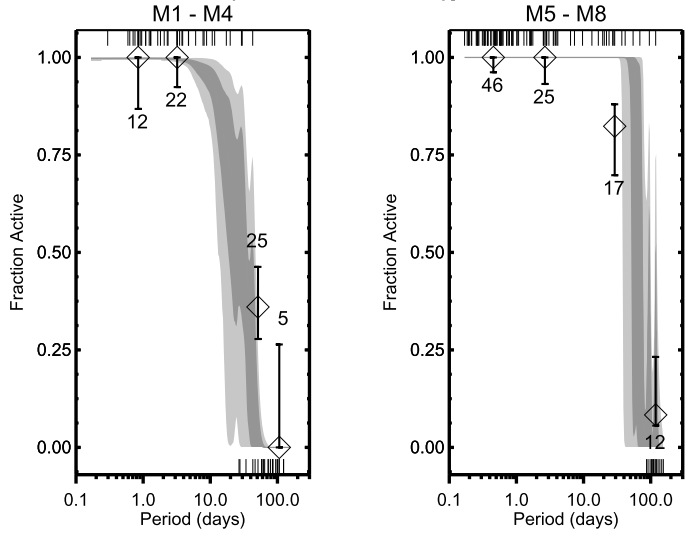
\includegraphics[width=.8\textwidth]{figures/mdwarfactivity.png}
  \caption{The fraction of active M dwarfs as a function of stellar rotation period
    for early-to-mid (\emph{left panel}) and mid-to-late (\emph{right panel}) M
    dwarfs. An individual star's activity flag is based on H$\alpha$ emission observations.
    The activity fraction of stars decreases as rotation slows although mid-to-late M
    dwarfs can maintain a higher activity fraction than early-to-mid M dwarfs within a given
    \prot{} bin. \citep[Image credit:][]{west15}}
  \label{fig:activity}
\end{figure}

Fig.~\ref{fig:rotation} depicts the rotation period
distribution of M dwarfs in the solar neighbourhood \citep{newton16a} and in the Kepler
field up to just $P_{\mathrm{rot}} < 70$ days \citep{mcquillan13a}.
Two distinct populations exist, namely a rapidly
rotating population (\prot{} $\lesssim 3$ days) and a slowly rotating population
(\prot{} $\gtrsim 50$ days). It has been proposed that these two populations
have a distinct range of ages with
the slow rotators belonging to an older stellar population based on their galactic
kinematics \citep{irwin11} and resulting from magnetic-braking over time.
Indeed, a fairly robust relation exists for GK and early M dwarf stars between stellar
mass, age, and rotation \citep[gyrochronology;][]{barnes03}. \\

\begin{figure}
  \centering
  %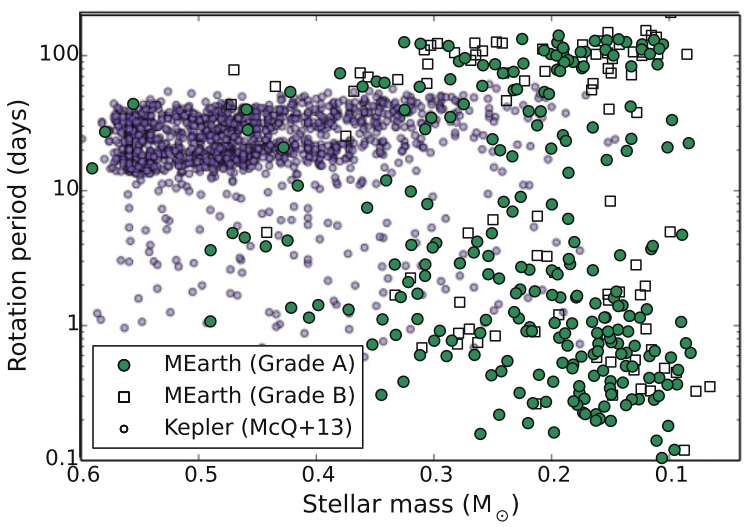
\includegraphics[width=.8\textwidth]{figures/mdwarfrotation.png}
  \caption{Rotation period versus stellar mass for solar neighbourhood and Kepler field
    M dwarfs. Periods of the Kepler stars are intentionally capped at \prot{} $=70$ days.
    The distribution of \prot{} appears to be bi-modal featuring a
    population of fast (\prot{} $\lesssim 3$ days) and slowly (\prot{} $\gtrsim 50$ days)
    rotating M dwarfs with a dearth of stars at intermediate \prot{.} These features are
    thought to be indicative of two differently aged populations. 
    \citep[Image credit:][]{newton16a}}
\label{fig:rotation}
\end{figure}

Another important point regarding active regions is that their lifetimes are comparable
to the stellar rotation timescale. This means that the associated stellar activity can vary
between rotation cycles. As seen in Fig.~\ref{fig:rotation},
the lifetimes can range from days to months \citep{schrijver02}. Active region
lifetimes are primarily determined by their sizes \citep{berdyugina05} as they
diffuse into the photosphere; larger volume/surface ratios results in longer lifetimes
\citep{petrovay97}.


\emph{Magnetic Cycles}:
the Sun undergoes a long-term magnetic cycle with an 11 year period as measured by the
fractional coverage or number of sunspots and faculae visible on its surface \citep{hathaway10}.
At solar maximum, the 
peak in magnetic activity over the solar cycle, the Sun i) experiences strong prominences
and coronal mass ejections and ii) contains a large number of active regions which contribute
to a higher level of activity in RV time series as well as in other observables
\citep{maunder04}. Long-term magnetic activity cycles have been observed in long-baseline
spectroscopic monitoring programs. From solar observations, the flux in the \caii{}
H and K lines are known to correlate with the number of sunspots. Numerous results from
similar surveys have
demonstrated that the majority of Sun-like stars do exhibit magnetic activity cycles
with a range of periods from $\sim 7-30$ years \citep{duncan91, lockwood97, balinunas98}. \\

As it pertains to RV planet searches, full activity cycles have yet
to be observed and precisely characterized. Subsections of the cyclic trends have been seen in
certain mature RV surveys to be correlated with
the $\log{R'_{\mathrm{HK}}}$ spectroscopic activity indicator \citep[e.g.][]{lovis11}.
A common tactic to correct for such long-term activity trends in RV time series is to use a linear
relation between the RVs and the contemporaneous $\log{R'_{\mathrm{HK}}}$ time series
\citep{dumusque12}. The corresponding RV signal from magnetic cycles can reach tens of \mps{.}
Luckily, when searching for
planets whose orbital timescales are much less than the period of the star's magnetic cycle, the
corresponding activity is not of much concern. \\


\section{Point-form Thesis: Introduction}
\begin{itemize}
\renewcommand\labelitemi{--}
\item~\ref{sect:exoplanets} \textbf{Exoplanets}: exoplanet sin the local universe are 
extremely abundant and quite diverse compared to the planets in our own solar system.
\item~\ref{sect:detection} \textbf{Methods of Detecting Exoplanets}: there exists a 
number of methods of detecting exoplanets, each with its own sensitivities and biases.
\item~\ref{sect:rv} \textbf{Exoplanet Detection via Stellar Radial Velocity}: the 
  gravitational influence of planetary companions on their host star induces a periodically
  varying Doppler shift that may be detectable and used to measure a exoplanet's minimum mass
  and orbital properties.
\item~\ref{sect:spectrograph} \textbf{Measuring Radial Velocities}: hi-resolution 
  spectrographs are used to measure the Doppler shift of stellar absorption features.
  The precision of such measurements is often impeded by sources of error from the
  instrumentation, counting statistics, telluric contamination, and stellar activity.
\end{itemize}
